\documentclass[dvipsnames, hidelinks]{beamer}

% Enables the use of colour.
\usepackage{xcolor}
% Syntax high-lighting for code. Requires Python's pygments.
\usepackage{minted}
% Enables the use of umlauts and other accents.
\usepackage[utf8]{inputenc}
% Diagrams.
\usepackage{tikz}
% Settings for captions, such as sideways captions.
\usepackage{caption}
% Symbols for units, like degrees and ohms.
\usepackage{gensymb}
% Latin modern fonts - better looking than the defaults.
\usepackage{lmodern}
% Allows for columns spanning multiple rows in tables.
\usepackage{multirow}
% Better looking tables, including nicer borders.
\usepackage{booktabs}
% More math symbols.
\usepackage{amssymb}
% More math layouts, equation arrays, etc.
\usepackage{amsmath}
% More math fonts, like mathbb.
\usepackage{amsfonts}
% More theorem environments.
\usepackage{amsthm}
% More column formats for tables.
\usepackage{array}
% Adjust the sizes of box environments.
\usepackage{adjustbox}
% Better looking single quotes in verbatim and minted environments.
\usepackage{upquote}
% Better blank space decisions.
\usepackage{xspace}
% Better looking tikz trees.
\usepackage{forest}
% URLs.
\usepackage{hyperref}
% For plotting.
\usepackage{pgfplots}

% Various tikz libraries.
% For drawing mind maps.
\usetikzlibrary{mindmap}
% For adding shadows.
\usetikzlibrary{shadows}
% Extra arrows tips.
\usetikzlibrary{arrows.meta}
% Old arrows.
\usetikzlibrary{arrows}
% Automata.
\usetikzlibrary{automata}
% For more positioning options.
\usetikzlibrary{positioning}
% Creating chains of nodes on a line.
\usetikzlibrary{chains}
% Fitting node to contain set of coordinates.
\usetikzlibrary{fit}
% Extra shapes for drawing.
\usetikzlibrary{shapes}
% For markings on paths.
\usetikzlibrary{decorations.markings}
% For advanced calculations.
\usetikzlibrary{calc}

% GMIT colours.
\definecolor{gmitblue}{RGB}{20,134,225}
\definecolor{gmitred}{RGB}{220,20,60}
\definecolor{gmitgrey}{RGB}{67,67,67}

% Change some style options.
\usetheme{metropolis}
\usemintedstyle{manni}
\setbeamercolor{structure}{fg=gmitblue}
\setbeamercolor{frametitle}{fg=white, bg=gmitred}
\setbeamercolor{alerted text}{fg=gmitblue}
\usefonttheme[onlymath]{serif}

% \citeurl can be used to a clickable short url to a slide as a reference.
\renewcommand\footnoterule{}
\newcommand{\citeurl}[1]{\let\thefootnote\relax\footnotetext{\tiny \textcolor{gmitgrey}{\href{http://#1}{#1}}}}

% A basic horizontal rule.
\newcommand{\hr}{\rule{\textwidth}{0.5pt}}

% Prevent minted from showing errors.
\makeatletter
\expandafter\def\csname PYGdefault@tok@err\endcsname{\def\PYGdefault@bc##1{{\strut ##1}}}
\makeatother

\begin{document}
  \title{Graph Theory}
  \subtitle{}
  \author{ian.mcloughlin@gmit.ie}
  \date{}

  \begin{frame}
    \titlepage
  \end{frame}

  \begin{frame}
    \frametitle{Topics}
    \tableofcontents
  \end{frame}

  %!TEX root = slides.tex


\section{Fundamentals}

\begin{frame}{Seven Bridges of K{\"o}nigsberg}
	\begin{center}
		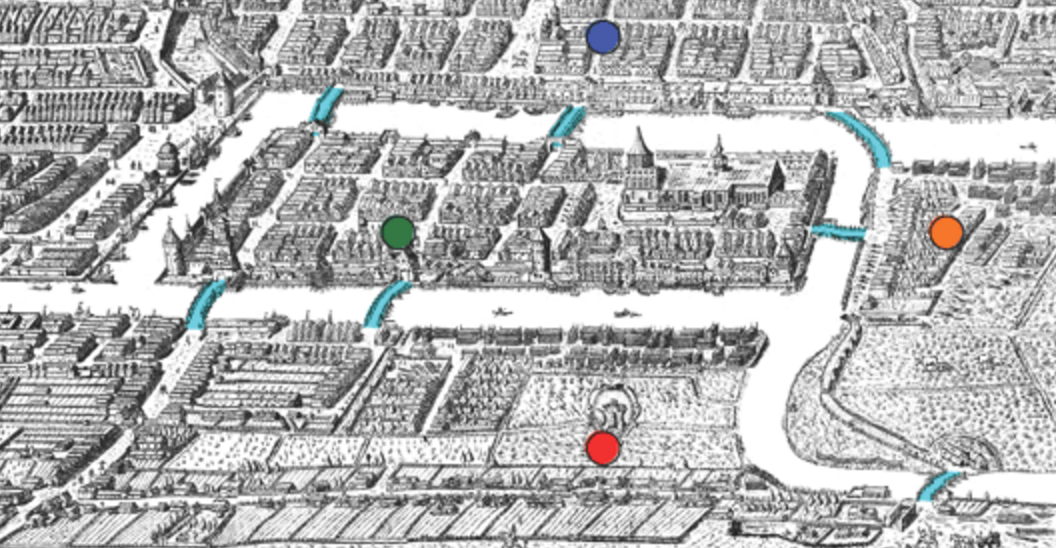
\includegraphics[width=9cm]{img/konigsberg.png}
	\end{center}
	Is it possible to walk through the city crossing each of the seven bridges once and only once?
		\citeurl{www.nature.com/nbt/journal/v29/n11}
\end{frame}

\begin{frame}{Leonhard Euler}
  \begin{columns}
    \begin{column}{0.25\textwidth}
      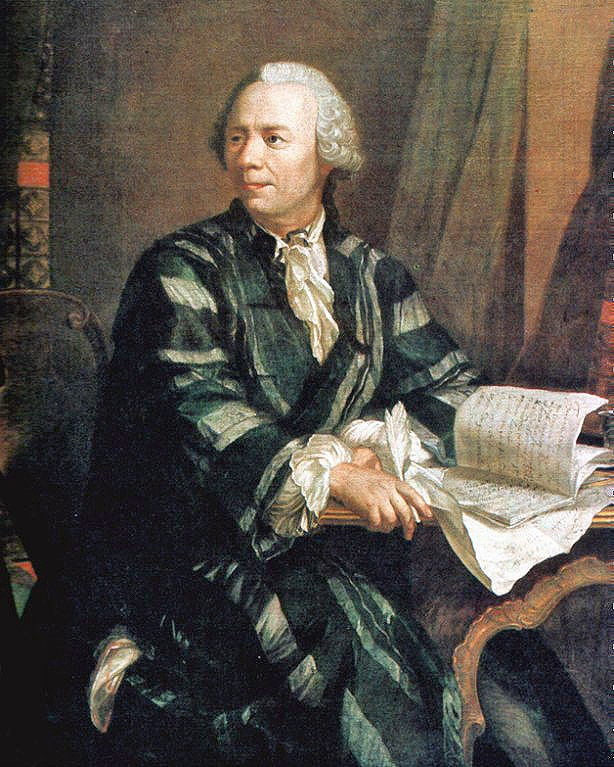
\includegraphics[height=1.8in]{img/euler.jpg}
    \end{column}
    \begin{column}{0.6\textwidth}
      \begin{itemize}
    	 \item Born 1707 in Basel, Switzerland.
        \vspace{0.25cm}
    	 \item Euler's identity: $\mathrm{e}^{i \pi} + 1 = 0$.
        \vspace{0.25cm}
    	 \item Solved the Bridges of K{\"o}nigsberg problem.
        \vspace{0.25cm}
        \item It's not possible to cross all bridges once and once only.
      \end{itemize}
    \end{column}
  \end{columns}
  \citeurl{https://en.wikipedia.org/wiki/Leonhard\_Euler}
\end{frame}

\begin{frame}{Graph of K{\"o}nigsberg}
  \begin{adjustbox}{max width={0.9\textwidth},center} 
    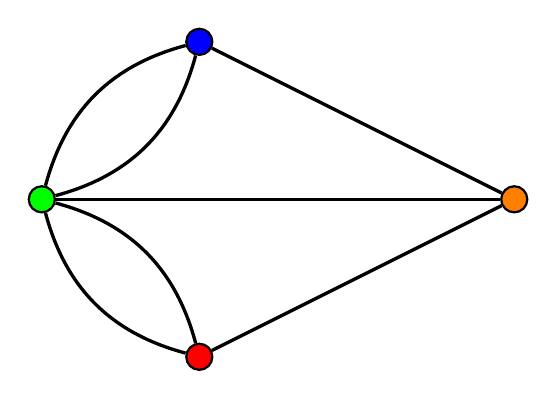
\begin{tikzpicture}
			\begin{scope}[every node/.style={circle,thick,draw}]
		    \node[fill=green] (A) at (0,0) {};
		    \node[fill=blue] (B) at (2,2) {};
		    \node[fill=orange] (C) at (6,0) {};
		    \node[fill=red] (D) at (2,-2) {};
			\end{scope}
			\begin{scope}[every edge/.style={draw=black,very thick}]
		    \path (A) edge[bend right=30] (B);
    		\path (A) edge[bend left=30] (B);
		    \path (A) edge[bend right=30] (D);
		    \path (A) edge[bend left=30]  (D);
		    \path (B) edge (C);
		    \path (A) edge (C);
		    \path (D) edge (C);
	    \end{scope}
    \end{tikzpicture}
  \end{adjustbox}
\end{frame}

\begin{frame}{Graph definition}
	\begin{definition}
	A \emph{graph} consists of a finite set $V$ and a set $E$ of 2-subsets of $V$.
	\end{definition}
	\vspace{0.5cm}
	\begin{description}
		\item[Vertices] -- the elements of the set $V$ are called vertices.
		\vspace{0.25cm}
		\item[Edges] -- the elements of $E$ are called edges.
		\vspace{0.25cm}
		\item[$G = (V,E)$] -- this is the way we write the graph $G$ consists of the vertex set $V$ and the edge set $E$.
	\end{description}
\end{frame}

\begin{frame}{Sets of K{\"o}nigsberg}
$$ V = \{Green, Blue, Orange, Red\} $$
\begin{align*}
E = \{&\\
			&\{Green, Blue\}, \{Green, Blue\}, \{Green, Red\},\\
      &\{Green, Red\}, \{Blue, Orange\}, \{Green, Orange\},\\
      &\{Red, Orange\}\\
      \}&
\end{align*}
\end{frame}

\begin{frame}{Adjanceny list}
	\begin{center}
	\begin{tabular}{c@{\hskip 0.5cm}c@{\hskip 0.5cm}c@{\hskip 0.5cm}c}
	Green & Blue & Orange & Red \\
  \midrule
	Blue & Green & Blue & Green \\
	Orange & Orange & Green & Orange \\
	Red & & Red & \\
	\end{tabular}
	\end{center}
\end{frame}

\begin{frame}{Defining different types of graphs}
	
	\begin{block}{Our definition of a graph}
	The definition given above for a graph is not consistent with looped edges, directed edges or repeated edges. We only need to make small changes to the definition of a graph to allow for directed edges and repeated edges.
	\end{block}
	
	\begin{description}
		\item[Repeated edges] are edges that start and end at the same vertices.
		\item[Directed edges] are edges where a direction is added.
		\item[Looped edges] begin and end at the same vertex.
	\end{description}
	
	The application will determine the definition we want to use.
\end{frame}


\begin{frame}{A better example}
  \begin{adjustbox}{max width={0.9\textwidth},center} 
    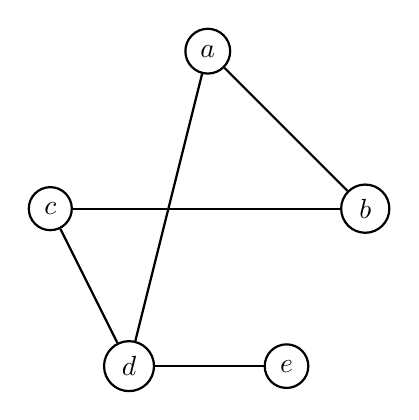
\begin{tikzpicture}
      \begin{scope}[every node/.style={circle,thick,draw}]
        \node (a) at (2,4) {$a$};
        \node (b) at (4,2) {$b$};
        \node (e) at (3,0) {$e$};
        \node (d) at (1,0) {$d$};
        \node (c) at (0,2) {$c$};
      \end{scope}
      \begin{scope}[every edge/.style={draw=black,thick}]
        \path (a) edge (b);
        \path (a) edge (d);
        \path (b) edge (c);
        \path (e) edge (d);
        \path (d) edge (c);
      \end{scope}
    \end{tikzpicture}
  \end{adjustbox}
  \vspace{0.1cm}
  \begin{block}{Exercise}
	Determine the vertex set, edge set and adacency list of this graph.
  \end{block}
  
  \citeurl{global.oup.com/booksites/content/9780198507185/}
\end{frame}


\begin{frame}{Another better example}
  \begin{adjustbox}{max width={0.9\textwidth},center} 
    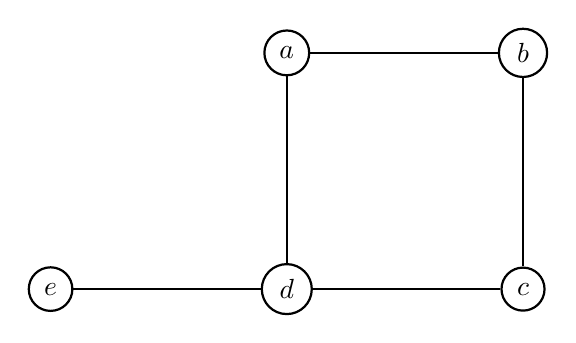
\begin{tikzpicture}
      \begin{scope}[every node/.style={circle,thick,draw}]
        \node (a) at (0,3) {$a$};
        \node (b) at (3,3) {$b$};
        \node (e) at (-3,0) {$e$};
        \node (d) at (0,0) {$d$};
        \node (c) at (3,0) {$c$};
      \end{scope}
      \begin{scope}[every edge/.style={draw=black,thick}]
        \path (a) edge (b);
        \path (a) edge (d);
        \path (b) edge (c);
        \path (e) edge (d);
        \path (d) edge (c);
      \end{scope}
    \end{tikzpicture}
  \end{adjustbox}
  \vspace{0.1cm}
  \begin{block}{Exercise}
	Determine the vertex set, edge set and adacency list of this graph.
  \end{block}
  
  \citeurl{global.oup.com/booksites/content/9780198507185/}
\end{frame}

\begin{frame}{Complete graph $K_n$}
  \begin{adjustbox}{max width={0.9\textwidth},center} 
    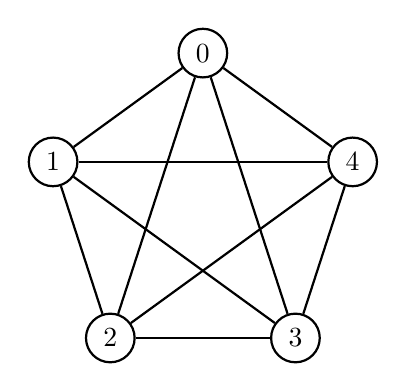
\begin{tikzpicture}
			\begin{scope}[every node/.style={circle,thick,draw}]
			\foreach \s in {0,...,4}
			{
				\node (\s) at ({72 * \s + 90}:2) {$\s$};
			}
			\end{scope}
      \begin{scope}[every edge/.style={draw=black,thick}]
        \path (0) edge (1);
				\path (0) edge (2);
				\path (0) edge (3);
				\path (0) edge (4);
        \path (1) edge (2);
        \path (1) edge (3);
        \path (1) edge (4);
        \path (2) edge (3);
				\path (2) edge (4);
				\path (3) edge (4);
      \end{scope}
    \end{tikzpicture}
  \end{adjustbox}
  \vspace{0.1cm}
  \begin{block}{Exercise}
	Determine the vertex set, edge set and adacency list of $K_5$.
  \end{block}
\end{frame}


\begin{frame}{Wheel graph $W_n$}
  \begin{adjustbox}{max width={0.9\textwidth},center} 
    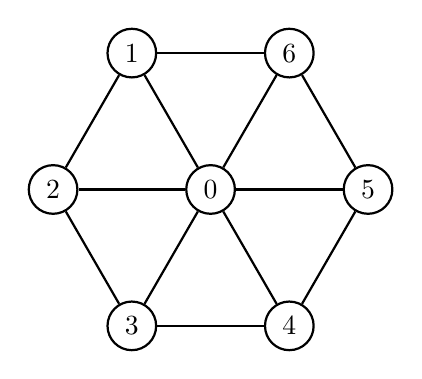
\begin{tikzpicture}
			\begin{scope}[every node/.style={circle,thick,draw}]
				\foreach \s in {1,...,6}
				{
					\node (\s) at ({60 * \s + 60}:2) {$\s$};
				}
				\node (0) at (0:0) {$0$};
			\end{scope}
      \begin{scope}[every edge/.style={draw=black,thick}]
        \path (0) edge (1);
				\path (0) edge (2);
				\path (0) edge (3);
				\path (0) edge (4);
        \path (0) edge (5);
        \path (0) edge (6);
        \path (1) edge (2);
        \path (2) edge (3);
				\path (3) edge (4);
				\path (4) edge (5);
				\path (5) edge (6);
				\path (6) edge (1);
      \end{scope}
    \end{tikzpicture}
  \end{adjustbox}
  \vspace{0.1cm}
  \begin{block}{Exercise}
	Determine the vertex set, edge set and adacency list of $W_6$.
  \end{block}
\end{frame}


\begin{frame}{Degree of a vertex}

	\begin{definition}
		The degree of a vertex is the number of edges that contain it.
	\end{definition}
	  
  \begin{center}
    \begin{columns}
      \begin{column}{0.2\textwidth}
        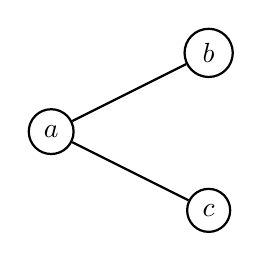
\begin{tikzpicture}
          \begin{scope}[every node/.style={circle,thick,draw}]
            \node (a) at (0,0) {$a$};
            \node (b) at (2,1) {$b$};
            \node (c) at (2,-1) {$c$};
          \end{scope}
          \begin{scope}[every edge/.style={draw=black,thick}]
            \path (a) edge (b);
            \path (a) edge (c);
          \end{scope}
        \end{tikzpicture}
      \end{column}
      \begin{column}{0.5\textwidth}
          The degree of the vertex $a$ is 2.
      \end{column}
    \end{columns}
  \end{center}

  \begin{block}{Exercise}
    For each of the vertices on the previous slide, determine its degree.
  \end{block}

\end{frame}


\begin{frame}{Functions}

	\begin{definition}
		Suppose that $X$ and $Y$ are sets.
		We say we have a function $f$ from $X$ to $Y$ if for each $x$ in $X$ we can specify a unique element in $Y$, which we denote by $f(x)$.
	\end{definition}

	\begin{center}
		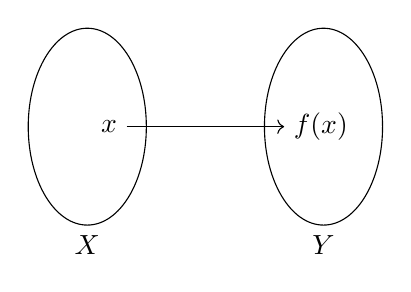
\begin{tikzpicture}
			\draw (0,0) ellipse (0.75 and 1.25);
			\draw (0,-1.5) node {$X$};
			\draw (3,0) ellipse (0.75 and 1.25);
			\draw (3,-1.5) node {$Y$};

			\draw [->]  (0.5,0) node[anchor=east] {$x$} -- (2.5,0) node[anchor=west] {$f(x)$};
		\end{tikzpicture}
	\end{center}

\end{frame}



\begin{frame}{Bijections}

	\begin{definition}
		A bijection is function $f$ from a set $X$ to a set $Y$ where both of the following are true:
			\begin{itemize}
				\item every $y$ in $Y$ is a value $f(x)$ for at most one $x$ in $X$.
				\item every $y$ in $Y$ is a value $f(x)$ for at least one $x$ in  $X$.
			\end{itemize}
	\end{definition}

	\begin{center}
		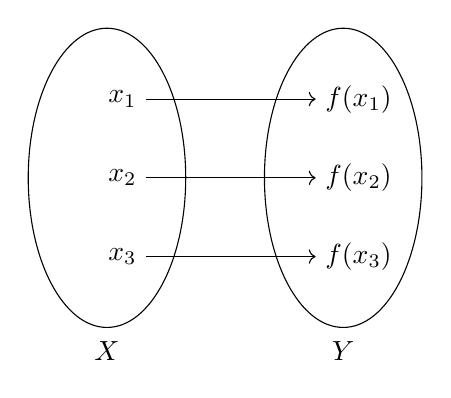
\begin{tikzpicture}
			\draw (0,0) ellipse (1 and 1.9);
			\draw (0,-2.2) node {$X$};
			\draw (3,0) ellipse (1 and 1.9);
			\draw (3,-2.2) node {$Y$};

			\draw [->]  (0.5,1) node[anchor=east] {$x_1$} -- (2.65,1) node[anchor=west] {$f(x_1)$};
			\draw [->]  (0.5,0) node[anchor=east] {$x_2$} -- (2.65,0) node[anchor=west] {$f(x_2)$};
			\draw [->]  (0.5,-1) node[anchor=east] {$x_3$} -- (2.65,-1) node[anchor=west] {$f(x_3)$};
		\end{tikzpicture}
	\end{center}

\end{frame}


\begin{frame}{Isomorphism}

	\begin{definition}
		Two graphs $G_1$ and $G_2$ are said to be isomorphic when there is a bijection $\alpha$ for the vertex set $V_1$ of $G_1$ to the vertex set $V_2$ of $G_2$ such that $\{\alpha (x) , \alpha (y) \}$ is an edge of $G_2$ if and only if $(x,y)$ is an edge of $G_1$.
	\end{definition}
	  
  \begin{center}
    \begin{columns}
      \begin{column}{0.3\textwidth}
        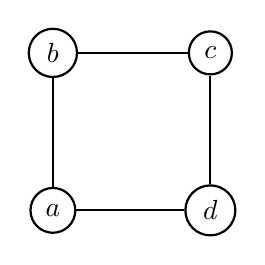
\begin{tikzpicture}
          \begin{scope}[every node/.style={circle,thick,draw}]
            \node (a) at (0,0) {$a$};
            \node (b) at (0,2) {$b$};
            \node (c) at (2,2) {$c$};
            \node (d) at (2,0) {$d$};
          \end{scope}
          \begin{scope}[every edge/.style={draw=black,thick}]
            \path (a) edge (b);
            \path (b) edge (c);
            \path (c) edge (d);
            \path (d) edge (a);
          \end{scope}
        \end{tikzpicture}
      \end{column}
      
      \begin{column}{0.3\textwidth}
        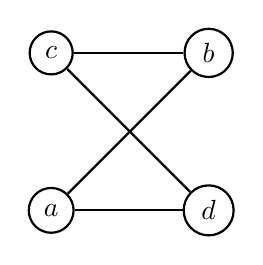
\begin{tikzpicture}
          \begin{scope}[every node/.style={circle,thick,draw}]
            \node (a) at (0,0) {$a$};
            \node (c) at (0,2) {$c$};
            \node (b) at (2,2) {$b$};
            \node (d) at (2,0) {$d$};
          \end{scope}
          \begin{scope}[every edge/.style={draw=black,thick}]
            \path (b) edge (c);
            \path (c) edge (d);
            \path (b) edge (a);
            \path (d) edge (a);
          \end{scope}
        \end{tikzpicture}
      \end{column}
      
      \begin{column}{0.3\textwidth}
        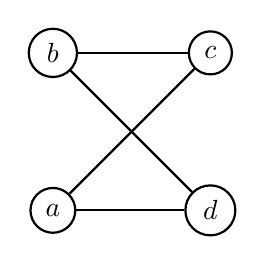
\begin{tikzpicture}
          \begin{scope}[every node/.style={circle,thick,draw}]
            \node (a) at (0,0) {$a$};
            \node (b) at (0,2) {$b$};
            \node (c) at (2,2) {$c$};
            \node (d) at (2,0) {$d$};
          \end{scope}
          \begin{scope}[every edge/.style={draw=black,thick}]
            \path (b) edge (c);
            \path (b) edge (d);
            \path (c) edge (a);
            \path (d) edge (a);
          \end{scope}
        \end{tikzpicture}
      \end{column}
    \end{columns}
  \end{center}

\end{frame}


\begin{frame}{Sum of degrees}

	\begin{theorem}
		The sum of the degrees of the vertices of a graph $G = (V,E)$ is equal to twice the number of edges:
			\[ \sum_{\mathrm{v} \in V} \delta (\mathrm{v}) = 2 | E | \]
	\end{theorem}

	\begin{columns}
		\begin{column}{0.75\textwidth}
			\begin{proof}
				The degree $\delta (\mathrm{v})$ of a vertex $\mathrm{v}$ is equal to the number of edges incident on it.
				Every edge is incident on two vertices.
				So every edge contributes $1$ to the degrees of two distinct vertices.
				Therefore every edge contributes $2$ to the sum total of the degrees of all the vertices.
			\end{proof}
		\end{column}
		\begin{column}{0.2\textwidth}
			\begin{center}
        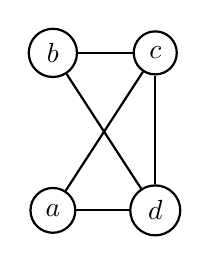
\begin{tikzpicture}
          \begin{scope}[every node/.style={circle,thick,draw}]
            \node (a) at (0,0) {$a$};
            \node (b) at (0,2) {$b$};
            \node (c) at (1.3,2) {$c$};
            \node (d) at (1.3,0) {$d$};
          \end{scope}
          \begin{scope}[every edge/.style={draw=black,thick}]
            \path (b) edge (c);
            \path (b) edge (d);
            \path (d) edge (c);
            \path (c) edge (a);
            \path (d) edge (a);
          \end{scope}
        \end{tikzpicture}
			\end{center}
		\end{column}
	\end{columns}
\end{frame}

\begin{frame}{Handshaking lemma}
	\begin{definition}
		A vertex is an odd vertex if its degree is odd, and it is an even vertex if its degree is even.
		The set of all odd vertices is denoted $V_o$ and the set of all even vertices is denoted $V_e$.
	\end{definition}
	\begin{center}
		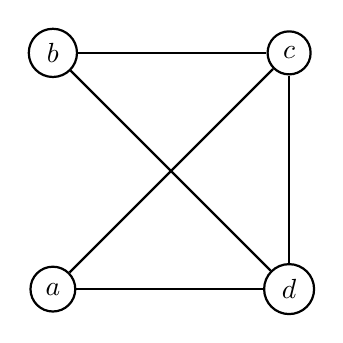
\begin{tikzpicture}
			\begin{scope}[every node/.style={circle,thick,draw}]
				\node (a) at (0,0) {$a$};
				\node (b) at (0,3) {$b$};
				\node (c) at (3,3) {$c$};
				\node (d) at (3,0) {$d$};
			\end{scope}
			\begin{scope}[every edge/.style={draw=black,thick}]
				\path (b) edge (c);
				\path (b) edge (d);
				\path (d) edge (c);
				\path (c) edge (a);
				\path (d) edge (a);
			\end{scope}
		\end{tikzpicture}
	\end{center}
	\begin{block}{Exercise}
		Which of the above vertices are even, and which are odd?
	\end{block}
\end{frame}

\begin{frame}{Handshaking lemma}

	\begin{lemma}
		The number of odd vertices $| V_o |$ in a graph is even.
	\end{lemma}

	\begin{proof}
		The sets $V_o$ and $V_e$ are disjoint (i.e.\ they don't have any elements in common.)
		Also, every vertex is either in $V_o$ or $V_e$.
		Therefore $V = V_o \cup V_e$ and $|V| = |V_o| + |V_e|$.
		
		Furthermore:
			\[ \sum_{\mathrm{v} \in V_o} \delta(\mathrm{v}) + \sum_{\mathrm{v} \in V_e} \delta(\mathrm{v}) = 2 |E| \]

		Both $2|E|$ and $\sum_{\mathrm{v} \in V_e} \delta(\mathrm{v})$ are even, so $\sum_{\mathrm{v} \in V_o} \delta(\mathrm{v})$ must be.
		Since $\delta(\mathrm{v})$ is odd for every $\mathrm{v}$ in $V_o$, this must mean that $|V_o|$ is even.
	\end{proof}

\end{frame}


\begin{frame}{Isomorphism: degrees}

	\begin{block}{Exercise}
		Determine if these two graphs are isomorphic.

		\begin{columns}
			\begin{column}{0.5\textwidth}
				\begin{center}
	        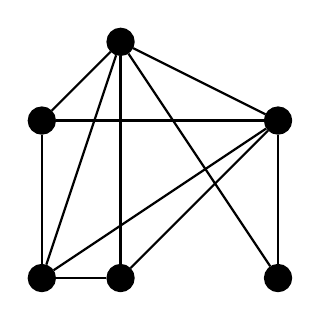
\begin{tikzpicture}
	          \begin{scope}[every node/.style={circle,thick,draw,fill}]
	            \node (a) at (0,1) {};
	            \node (b) at (0,4) {};
	            \node (c) at (2,1) {};
	            \node (d) at (2,3) {};
	            \node (e) at (-1,1) {};
	            \node (f) at (-1,3) {};
	          \end{scope}
	          \begin{scope}[every edge/.style={draw=black,thick}]
	            \path (a) edge (b);
	            \path (a) edge (d);
	            \path (a) edge (e);
	            \path (b) edge (c);
	            \path (b) edge (d);
 	            \path (b) edge (e);
 	            \path (b) edge (f);
 	            \path (c) edge (d);
 	            \path (d) edge (e);           
 	            \path (d) edge (f);
 	            \path (e) edge (f);
	          \end{scope}
	        \end{tikzpicture}
				\end{center}
			\end{column}
			\begin{column}{0.5\textwidth}
				\begin{center}
	        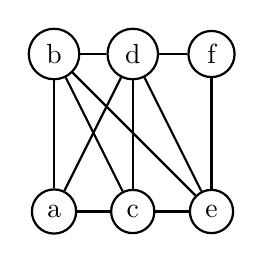
\begin{tikzpicture}
	          \begin{scope}[every node/.style={circle,thick,draw}]
	            \node (a) at (0,0) {a};
	            \node (b) at (0,2) {b};
	            \node (c) at (1,0) {c};
	            \node (d) at (1,2) {d};
	            \node (e) at (2,0) {e};
	            \node (f) at (2,2) {f};
	          \end{scope}
	          \begin{scope}[every edge/.style={draw=black,thick}]
	            \path (a) edge (b);
	            \path (a) edge (c);
	            \path (c) edge (e);
	            \path (a) edge (d);
	            \path (b) edge (c);
	            \path (b) edge (d);
 	            \path (b) edge (e);
 	            \path (b) edge (d);
 	            \path (d) edge (f);
 	            \path (c) edge (d);
 	            \path (d) edge (e);	            
 	            \path (e) edge (f);
	          \end{scope}
	        \end{tikzpicture}
				\end{center}
			\end{column}
		\end{columns}
	\end{block}
\end{frame}


\begin{frame}{Directed graph definition}
	\begin{definition}
	A \emph{directed graph} consists of a finite set $V$ and a set $E$ of 2-tuples (ordered pairs of elements) from $V$.
	\end{definition}
	\vspace{0.2cm}
	\begin{description}
		\item[Looped edges] are allowed in this definition. A single one per vertex.
		\item[Multiple edges] between the same start and end vertices are not allowed. However, two edges are allowed between every pair of vartices so long as they have opposite directions.
		\item[Direct edges] use round brackets rather than curly braces: $E = \{ (a,b) \mid a,b \in V\}$.
	\end{description}
\end{frame}


\begin{frame}{Multigraph definition}
	\begin{definition}
	A \emph{multigraph} consists of a finite set $V$ and a multiset $E$ of 2-subsets from $V$.
	\end{definition}
	\vspace{0.2cm}
	\begin{description}
		\item[Multisets] are like sets, but the same element can be in the set more than once.
		\item[Directed multigraphs] are similar, but $E$ is a set of 2-tuples of elements in $V$.
	\end{description}
\end{frame}
  %!TEX root = slides.tex

\section{Trees}


\begin{frame}{Definition}
  
  \begin{block}{Tree}
    A \emph{tree} is a graph where every pair of vertices has a path between them, and there are no cycles.
  \end{block}
  
  \begin{columns}
    \begin{column}{0.5\textwidth}
      \begin{center}
        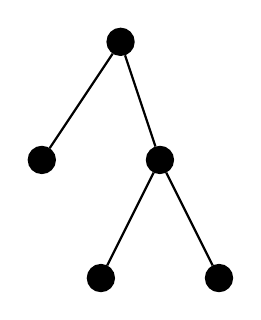
\begin{tikzpicture}
        \begin{scope}[every node/.style={circle,thick,draw,fill}]
        \node (a) at (1.5,3) {};
        \node (b) at (0.5,1.5) {};
        \node (c) at (2,1.5) {};
        \node (d) at (1.25,0) {};
        \node (e) at (2.75,0) {};
        \end{scope}
        \begin{scope}[every edge/.style={draw=black,thick}]
        \path (a) edge (b);
        \path (a) edge (c);
        \path (c) edge (d);
        \path (c) edge (e);
        \end{scope}
        \end{tikzpicture}
      \end{center}
    \end{column}
    \begin{column}{0.5\textwidth}
      \begin{center}
        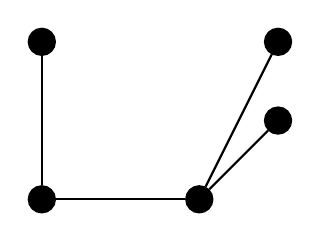
\begin{tikzpicture}
        \begin{scope}[every node/.style={circle,thick,draw,fill}]
        \node (a) at (0,3) {};
        \node (b) at (0,1) {};
        \node (c) at (2,1) {};
        \node (d) at (3,2) {};
        \node (e) at (3,3) {};
        \end{scope}
        \begin{scope}[every edge/.style={draw=black,thick}]
        \path (a) edge (b);
        \path (b) edge (c);
        \path (c) edge (d);
        \path (c) edge (e);
        \end{scope}
        \end{tikzpicture}
      \end{center}
    \end{column}
  \end{columns}
\end{frame}

\begin{frame}{Levels}
  \begin{description}
    \item[Root] Specified vertex for some purpose.
    \item[Levels] Root is at level 0, neighbours of the root are at level 1, their other neighbours at level 2, and so on.
    \item[Height] $h$, where vertex at level $h$ but not at level $h+1$.
    \item[Leaf] Vertex at level $i$ with no neighbours at level $i+1$.
    \item[Internal vertex] A non-leaf.
  \end{description}
  \vspace{0.5cm}
  \begin{center}
    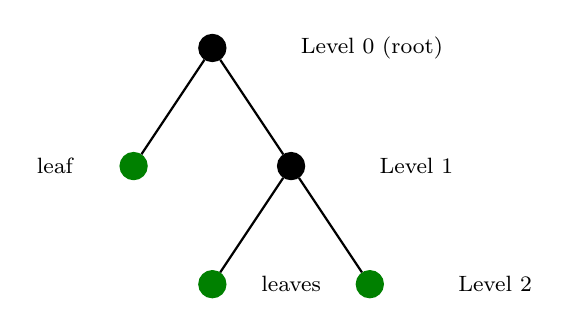
\begin{tikzpicture}
    \begin{scope}[every node/.style={circle,thick,draw,fill}]
      \node (a) at (1.5,3) {};
      \node (b)[green!50!black] at (0.5,1.5) {};
      \node (c) at (2.5,1.5) {};
      \node (d)[green!50!black] at (1.5,0) {};
      \node (e)[green!50!black] at (3.5,0) {};
    \end{scope}
    \node () [right of=a, anchor=west] {\footnotesize Level 0 (root)};
    \node () [right of=c, anchor=west] {\footnotesize Level 1};
    \node () [right of=e, anchor=west] {\footnotesize Level 2};
    \node () [left of=b] {\footnotesize leaf};
    \node () [left of=e] {\footnotesize leaves};
    \begin{scope}[every edge/.style={draw=black,thick}]
      \path (a) edge (b);
      \path (a) edge (c);
      \path (c) edge (d);
      \path (c) edge (e);
    \end{scope}
    \end{tikzpicture}
  \end{center}
\end{frame}

\begin{frame}{$m$-ary Rooted Tree}
  \begin{definition}
    When a vertex at level $i$ is connected to a vertex at level $i+1$ it's common to call the former the \emph{father} and the latter the \emph{son}.
    A rooted tree is $m$-ary if every father has the same number of sons.
    A $2$-ary rooted tree is called a \emph{binary tree}.
  \end{definition}
  \begin{center}
    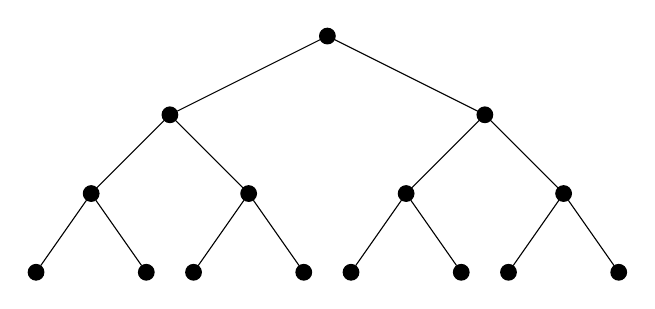
\begin{tikzpicture}
    \begin{scope}[every node/.style={circle,draw,fill,scale=0.6}]
    \node (a) at (3,4) {};
    \node (b) at (1,3) {};
    \node (c) at (5,3) {};
    \node (d) at (0,2) {};
    \node (e) at (2,2) {};
    \node (f) at (4,2) {};
    \node (g) at (6,2) {};
    \node (h) at (-0.7,1) {};
    \node (i) at (0.7,1) {};
    \node (j) at (1.3,1) {};
    \node (k) at (2.7,1) {};
    \node (l) at (3.3,1) {};
    \node (m) at (4.7,1) {};
    \node (n) at (5.3,1) {};
    \node (o) at (6.7,1) {};
    \end{scope}
    \begin{scope}[every edge/.style={draw=black}]
    \path (a) edge (b);
    \path (a) edge (c);
    \path (b) edge (d);
    \path (b) edge (e);
    \path (c) edge (f);
    \path (c) edge (g);
    \path (d) edge (h);
    \path (d) edge (i);
    \path (e) edge (j);
    \path (e) edge (k);
    \path (f) edge (l);
    \path (f) edge (m);
    \path (g) edge (n);
    \path (g) edge (o);
    \end{scope}
    \end{tikzpicture}
  \end{center}
\end{frame}

\begin{frame}{Isomorphic Rooted Trees}
  \begin{definition}
   Two rooted trees are said to be \emph{isomorphic} if there is an isomorphism between them which takes the root of one tree to the root of the other.
  \end{definition}
\end{frame}

\begin{frame}{Height of an $m$-ary rooted tree}
  
  \begin{theorem}
    The height $h$ of an $m$-ary rooted tree with $l$ leaves is at least $\log_m l$.
    That is:
    \[ h \geq \log_m l \]
  \end{theorem}
  
  \begin{proof}
    First note that: $h \geq log_m l \hspace{0.1cm} \Leftrightarrow \hspace{0.1cm} m^h \geq m^{log_m l} \hspace{0.1cm} \Leftrightarrow \hspace{0.1cm} m^h \geq l$.
    
    So, we just need to show the number of leaves is at most $m^h$.
    For a tree of depth 0, there is only one vertex and $m^0 \leq 1$.
    Suppose we know that the theorem is true for trees of height $h-1$.
    Consider a tree of height $h$, with $l$ leaves.
    We can create $m$ trees of height $h-1$ from it by deleting the root.
    Each of these smaller trees has at most $m^{h-1}$ leaves, and there are $m$ of them.
    So the big tree has at most $m \times m^{h-1} = m^h$ leaves.

  \end{proof}
  
\end{frame}
  %!TEX root = slides.tex


\section{Graph databases}


\begin{frame}{Digraph definition}
  \begin{definition}
    A \emph{digraph} (short for directional graph) consists of a finite set $V$ and a set $E$ of ordered pairs of elements of $V$.
  \end{definition}
  \vspace{0.25cm}
  \begin{description}
    \item[Degrees] of vertices can now be split into in-degrees and out-degrees.
    \item[Walks, paths, cycles] must be redefined.
    \item[Loops] are allowed in the above definition, unless we rule them out.
  \end{description}
\end{frame}


\begin{frame}{Digraph example}
  \begin{center}
    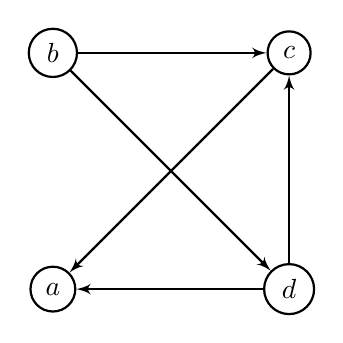
\begin{tikzpicture}
    \begin{scope}[every node/.style={circle,thick,draw}]
    \node (a) at (0,0) {$a$};
    \node (b) at (0,3) {$b$};
    \node (c) at (3,3) {$c$};
    \node (d) at (3,0) {$d$};
    \end{scope}
    \begin{scope}[every edge/.style={draw=black,thick}]
    \path (b) edge[->,> = latex'] (c);
    \path (b) edge[->,> = latex'] (d);
    \path (d) edge[->,> = latex'] (c);
    \path (c) edge[->,> = latex'] (a);
    \path (d) edge[->,> = latex'] (a);
    \end{scope}
    \end{tikzpicture}
  \end{center}
\end{frame}

\begin{frame}{Neo4j}
    \begin{columns}
      \begin{column}{0.25\textwidth}
        
\includegraphics[height=1.8in]{img/neo4j.png}
      \end{column}
      \begin{column}{0.6\textwidth}
        \begin{itemize}
          \item Neo4j is an open-source NoSQL graph database implemented in Java and Scala.
          \vspace{0.25cm}
          \item Development started in 2003, it has been publicly available since 2007
          \vspace{0.25cm}
          \item Available on GitHub.
          \vspace{0.25cm}
          \item A graph is composed of two elements: a node and a relationship.
        \end{itemize}
      \end{column}
    \end{columns}
    \citeurl{http://neo4j.com/developer/graph-database/}
\end{frame}


\begin{frame}{Cypher}
  \begin{columns}
    \begin{column}{0.25\textwidth}
      
\includegraphics[height=1.8in]{img/neo4j.png}
    \end{column}
    \begin{column}{0.6\textwidth}
      \begin{itemize}
        \item Cypher is a declarative graph query language.
        \vspace{0.25cm}
        \item What to retrieve from a graph, not on how to retrieve it.
        \vspace{0.25cm}
        \item Allows for expressive and efficient querying and updating of the graph store.
        \vspace{0.25cm}
        \item Cypher borrows its structure from SQL.
      \end{itemize}
    \end{column}
  \end{columns}
  \citeurl{http://neo4j.com/docs/stable/cypher-introduction.html}
\end{frame}


\begin{frame}[fragile]{Cypher: Nodes}
  Create a node with the label User, and two properties:
  \begin{minted}[linenos, frame=lines, framesep=2mm]{cypher}
CREATE (user:User { Id: 123, Name: "Jim" });
  \end{minted}
  \vspace{1cm}
  Find the node(s) with label User and their Id property being 123:
  \begin{minted}[linenos, frame=lines, framesep=2mm]{cypher}
MATCH (user:User)
WHERE user.Id = 123
RETURN user;
  \end{minted}
  \citeurl{neo4j.com/docs/stable/cypher-query-lang.html}
\end{frame}

\begin{frame}[fragile]{Cypher: Relationships}
  Create a relationship with label FOLLOWS from user(s) with Id 123 to user(s) with Id 456: 
  \begin{minted}[linenos, frame=lines, framesep=2mm]{cypher}
MATCH (user1:User), (user2:User)
WHERE user1.Id = 123 AND user2.Id = 456
CREATE user1-[:FOLLOWS]->user2;
  \end{minted}
  \citeurl{neo4j.com/docs/stable/cypher-query-lang.html}
\end{frame}

\begin{frame}[fragile]{Cypher: Relationships and Nodes}
  Create a relationship with label INVITED from user(s) with Id 123 to a new user with Id 789 and Name Jack: 
  \begin{minted}[linenos, frame=lines]{cypher}
MATCH (invitee:User)
WHERE invitee.Id = 123
CREATE invitee-[:INVITED]->(invited:User {Id: 789,
                                        Name: "Jack"});
  \end{minted}
  \citeurl{neo4j.com/docs/stable/cypher-query-lang.html}
\end{frame}


\begin{frame}[fragile]{Cypher: DELETE}
  Delete all nodes: 
  \begin{minted}[linenos, frame=lines]{cypher}
MATCH (x)
DELETE x;
  \end{minted}
  \citeurl{neo4j.com/docs/stable/cypher-query-lang.html}
\end{frame}

\begin{frame}{Labels and properties}
  \begin{itemize}
    \item Suppose we have nodes representing people.
    \item We give them the label People.
    \item We also want to identify each person as either Male or Female.
    \item Should we use Male and Female labels, or a Gender property?
    \item If you are going to use the person's gender in a lot of queries, a normal property will be relatively slow, so you should use a label.
    \item However, you can also index some of your properties to high-light them as important.
    
  \end{itemize}
  \citeurl{neo4j.com/docs/stable/cypher-query-lang.html}
\end{frame}

\begin{frame}[fragile]{Cypher: shortestPath}
  Find the minimum number of hops betweem two nodes.
  \begin{minted}[linenos, frame=lines]{cypher}
MATCH p=shortestPath(
  (a:Actor {id: 1})-[*]-(b:Actor {id: 10})
  )
RETURN p;
  \end{minted}
  \citeurl{neo4j.com/docs/stable/cypher-query-lang.html}
\end{frame}


  %!TEX root = slides.tex

\section{Algorithms}

\begin{frame}{Decision tree}
  \begin{description}
    \item[Decision trees] are rooted trees where each vertex represents a decision.
    \vspace{2mm}
    \item[Possible results] of each decision are represented by the edges.
    \vspace{2mm}
    \item[These edges] connect the decision vertex to the vertices representing the outcomes, at the next level down.
    \vspace{2mm}
    \item[These vertices] is turn can represent more decisions.
    \vspace{2mm}
    \item[Final outcomes] of the procedure are represented by the leaves.
  \end{description}
\end{frame}

\begin{frame}[fragile]{Decision tree example}

  \begin{center}
    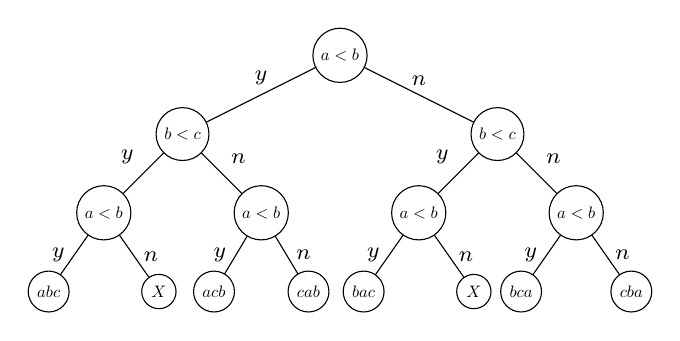
\begin{tikzpicture}
    \begin{scope}[every node/.style={circle,draw,scale=0.6}]
    \node (a) at (3,4) {$a<b$};
    \node (b) at (1,3) {$b<c$};
    \node (c) at (5,3) {$b<c$};
    \node (d) at (0,2) {$a<b$};
    \node (e) at (2,2) {$a<b$};
    \node (f) at (4,2) {$a<b$};
    \node (g) at (6,2) {$a<b$};
    \node (h) at (-0.7,1) {$abc$};
    \node (i) at (0.7,1) {$X$};
    \node (j) at (1.4,1) {$acb$};
    \node (k) at (2.6,1) {$cab$};
    \node (l) at (3.3,1) {$bac$};
    \node (m) at (4.7,1) {$X$};
    \node (n) at (5.3,1) {$bca$};
    \node (o) at (6.7,1) {$cba$};
    \end{scope}
    \begin{scope}[every edge/.style={draw=black}]
    \path (a) edge node[above] {\footnotesize $y$} (b);
    \path (a) edge node[above] {\footnotesize $n$} (c);
    \path (b) edge node[above left] {\footnotesize $y$} (d);
    \path (b) edge node[above right]  {\footnotesize $n$} (e);
    \path (c) edge node[above left] {\footnotesize $y$} (f);
    \path (c) edge node[above right]  {\footnotesize $n$} (g);
    \path (d) edge node[left] {\footnotesize $y$} (h);
    \path (d) edge node[right]  {\footnotesize $n$} (i);
    \path (e) edge node[left] {\footnotesize $y$} (j);
    \path (e) edge node[right]  {\footnotesize $n$} (k);
    \path (f) edge node[left] {\footnotesize $y$} (l);
    \path (f) edge node[right]  {\footnotesize $n$} (m);
    \path (g) edge node[left] {\footnotesize $y$} (n);
    \path (g) edge node[right]  {\footnotesize $n$} (o);
    \end{scope}
    \end{tikzpicture}
  \end{center}
\end{frame}

\begin{frame}{Height of a decision tree}
  \begin{description}
    \item[The height] of a decision tree is the maximum distance from root to leaf (as usual).
    \vspace{2mm}
    \item[Each] internal vertex represents a decision.
    \vspace{2mm}
    \item[The height] therefore is the maximium number of decisions made when starting from the root of the tree.
  \end{description}
\end{frame}

\end{document}
 